\documentclass[12pt, a4paper]{article}
\usepackage{graphicx} % Required for inserting images
\usepackage[paper=a4paper,top=1in,bottom=1in,right=1in,left=1in]{geometry}% http://ctan.org/pkg/geometry
\usepackage{amsmath, xparse}
\setcounter{MaxMatrixCols}{20}
\usepackage{caption}
\usepackage[framed, numbered]{matlab-prettifier}
\usepackage{longtable}
\usepackage{float}


\setlength\parindent{0pt}
\numberwithin{equation}{section}



\begin{document}

\begin{titlepage}
   \begin{center}
       
\includegraphics[width=0.25\textwidth]{img/metu.png}\\
       \vspace*{1cm}
       \Large
       \textbf{MIDDLE EAST TECHNICAL UNIVERSITY}\\
       \vspace{0.05cm}
       \textbf{DEPARTMENT OF MECHANICAL ENGINEERING}\\
       \vspace{1.2cm}
       \textbf{ME 310 – NUMERICAL METHODS}\\
       \textbf{SPRING 2022}\\
       \vspace{3cm}
       \text{HOMEWORK 2}\\
       \vspace{2cm}
       \text{Muhammed Rüstem ŞEVİK - 2446888}

       \vfill
       
       \small
       I understand that this is an individual assignment. I affirm that I have not given or received
any unauthorized help on this assignment, and that this work is my own.
            
       \vspace{0cm}

            
   \end{center}
\end{titlepage}

\newpage
    \renewcommand{\contentsname}{Table of Contents}
    \tableofcontents
    \listoffigures
    \listoftables
\newpage

\section{Introduction}

In this report the aim is to construct several numerical optimization codes by using MATLAB. The second question is about golden section search, quadratic interpolation and newtons method. The third question is about graphical solution and random search and the last question is about construction of a gradient based minimization method.

\section{Body}
\subsection{Question 2}
The question is to find the maximum of the growth rate by using golden section search, quadratic interpolation and the Newtons's method.
The function is:
\begin{equation}
g(c) = \frac{5c}{5+0.8c+c^2+0.2c^3}
\end{equation}

\subsubsection{Part A}

To find the value of $c$ at which the growth rate is maximized using the golden section search, we start with an interval of $[0,10]$. We will perform iterations until the interval width reduces down to $0.01$.

At the first iteration, we use the following initial values:
\begin{equation}
\begin{align}
x_L &= 0 \\
x_U &= 10 \\
R &= \frac{\sqrt{5} - 1}{2}\\
d &= R(x_U - x_L)\\
x_1 &= x_L + d\\
x_2 &= x_U - d\\
g_1 &= \frac{5x_1}{5 + 0.8x_1 + x_1^2 + 0.2x_1^3}\\
g_2 &= \frac{5x_2}{5 + 0.8x_2 + x_2^2 + 0.2x_2^3}\\
\end{align}
\end{equation}

Evaluate the numerical values:

\begin{equation}
\begin{align}
x_L &= 0 \\
x_U &= 10 \\
R &= 0.6180\\
d &= 6.180340\\
x_1 &= 6.180340\\
x_2 &= 3.819660\\
g_1 &= 0.324072\\
g_2 &= 0.565186 \\
\end{align}
\end{equation}

The second iteration. $g_1 < g_2$, the optimal value of $c$ must be in the interval $[x_L, x_2]$. In this case, we update our values as follows:
\begin{equation}
\begin{align}
x_U &= x_1\\
x_1 &= x_2\\
x_2 &= x_U - Rd\\
g_1 &= g_2\\
g_2 &= \frac{5x_2}{5 + 0.8x_2 + x_2^2 + 0.2x_2^3}\\
\end{align}
\end{equation}
Evaluate the numerical values:

\begin{equation}
\begin{align}
x_L &= 0 \\
x_U &= 6.180340 \\
d &= 3.819660\\
x_1 &= 3.819660\\
x_2 &= 2.360680\\
g_1 &= 0.565186\\
g_2 &= 0.782072 \\
\end{align}
\end{equation}

The third iteration. $g_1 < g_2$, the optimal value of $c$ must be in the interval $[x_L, x_2]$. In this case, we update our values as follows:
\begin{equation}
\begin{align}
x_U &= x_1\\
x_1 &= x_2\\
x_2 &= x_U - Rd\\
g_1 &= g_2\\
g_2 &= \frac{5x_2}{5 + 0.8x_2 + x_2^2 + 0.2x_2^3}\\
\end{align}
\end{equation}
Evaluate the numerical values:

\begin{equation}
\begin{align}
x_L &= 0 \\
x_U &= 3.819660 \\
d &= 3.819660\\
x_1 &= 2.360680\\
x_2 &= 1.458980\\
g_1 &= 0.782072\\
g_2 &= 0.818095 \\
\end{align}
\end{equation}

The following tabulated data contain all the iteration details where the $d > 0.01$ 


\begin{longtable}{cccccccccc}
  \caption{Details of iterations for golden section search method} \\
  \hline
  Iter      &   $x_L$    &    $x_U$  &     $x_1$  &  $x_2$  &  $g_1$  &  $g_2$  &  $d$ \\ \hline
  \endfirsthead

  \multicolumn{10}{c}%
  {\tablename\ \thetable\ -- \textit{Continued from previous page}} \\
  \hline
  Iter      &   $x_L$    &    $x_U$  &     $x_1$  &  $x_2$  &  $g_1$  &  $g_2$  &  $d$ \\ \hline
  \endhead

  \hline \multicolumn{10}{r}{\textit{Continued on next page}} \\
  \endfoot

  \hline
  \endlastfoot

        1 &  0.000000 &  10.000000 &  6.180340 &  3.819660 &  0.324072 &  0.565186 &  6.180340 \\ 
        2 &  0.000000 &  6.180340 &  3.819660 &  2.360680 &  0.565186 &  0.782072 &  3.819660 \\ 
        3 &  0.000000 &  3.819660 &  2.360680 &  1.458980 &  0.782072 &  0.818095 &  2.360680 \\ 
        4 &  0.000000 &  2.360680 &  1.458980 &  0.901699 &  0.818095 &  0.674819 &  1.458980 \\ 
        5 &  0.901699 &  2.360680 &  1.803399 &  1.458980 &  0.829684 &  0.818095 &  0.901699 \\ 
        6 &  1.458980 &  2.360680 &  2.016261 &  1.803399 &  0.818443 &  0.829684 &  0.557281 \\ 
        7 &  1.458980 &  2.016261 &  1.803399 &  1.671843 &  0.829684 &  0.830349 &  0.344419 \\ 
        8 &  1.458980 &  1.803399 &  1.671843 &  1.590537 &  0.830349 &  0.827802 &  0.212862 \\ 
        9 &  1.590537 &  1.803399 &  1.722093 &  1.671843 &  0.830750 &  0.830349 &  0.131556 \\ 
        10 &  1.671843 &  1.803399 &  1.753149 &  1.722093 &  0.830583 &  0.830750 &  0.081306 \\ 
        11 &  1.671843 &  1.753149 &  1.722093 &  1.702899 &  0.830750 &  0.830697 &  0.050250 \\ 
        12 &  1.702899 &  1.753149 &  1.733955 &  1.722093 &  0.830723 &  0.830750 &  0.031056 \\ 
        13 &  1.702899 &  1.733955 &  1.722093 &  1.714761 &  0.830750 &  0.830744 &  0.019194 \\ 
        14 &  1.714761 &  1.733955 &  1.726624 &  1.722093 &  0.830745 &  0.830750 &  0.011862 \\ 
        15 &  1.714761 &  1.726624 &  1.722093 &  1.719292 &  0.830750 &  0.830750 &  0.007331 \\ 
        16 &  1.719292	& 1.726624	& 1.723823	& 1.722093	& 0.830749	& 0.830750	& 0.004531	\\ 

\end{longtable}


\subsubsection{Part B}
The end points of the interval are given. Third point is the middle point of the interval. The inital points are as follows:

\begin{equation}
\begin{align}
x_0 &= 0 \\
x_1 &= 10 \\
x_2 &= 5    
\end{align}
\end{equation}

The quadratic interpolation formula is as follows:
\begin{equation}
    x_3=X_3(x_0,x_1,x_2)=\frac{f\left(x_0\right)\left(x_1^2-x_2^2\right)+f\left(x_1\right)\left(x_2^2-x_0^2\right)+f\left(x_2\right)\left(x_0^2-x_1^2\right)}{2 f\left(x_0\right)\left(x_1-x_2\right)+2 f\left(x_1\right)\left(x_2-x_0\right)+2 f\left(x_2\right)\left(x_0-x_1\right)}
\end{equation}

The first iteration:
\begin{equation}
\begin{align}
x_0 &= 0 \\
x_1 &= 10 \\
x_2 &= 5  \\
x_3 &= X_3(x_0,x_1,x_2)\\
f_0 &= f(x_0) \\
f_1 &= f(x_1) \\
f_2 &= f(x_2) \\
f_3 &= f(x_3) \\
\end{align}
\end{equation}

Evaluate the numerical values:

\begin{equation}
\begin{align}
x_0 &= 0 \\
x_1 &= 10 \\
x_2 &= 5  \\
x_3 &= 5.580709\\
f_0 &= 0 \\
f_1 &= 0.159744 \\
f_2 &= 0.423729 \\
f_3 &= 0.370219 \\
\end{align}
\end{equation}
Since the $x_3 > x_2$ and $f_3 < f_2$ we discard the $x_1$ and update as $x_1 = x_3$ similarly stated in the second iteration.\\
The second iteration:
\begin{equation}
\begin{align}
x_0 &= x_0 \\
x_1 &= x_3 \\
x_2 &= x_2  \\
x_3 &= X_3(x_0,x_1,x_2)\\
f_0 &= f(x_0) \\
f_1 &= f(x_1) \\
f_2 &= f(x_2) \\
f_3 &= f(x_3) \\
\end{align}
\end{equation}

Evaluate the numerical values:

\begin{equation}
\begin{align}
x_0 &= 0 \\
x_1 &= 5.580709 \\
x_2 &= 5  \\
x_3 &= 3.836814\\
f_0 &= 0 \\
f_1 &= 0.370219 \\
f_2 &= 0.423729 \\
f_3 &= 0.562796 \\
\end{align}
\end{equation}
Since the $x_3 < x_2$ and $f_3 > f_2$ we discard the $x_1$ and update as $x_1 = x_2$ and $x_2 = x_3$ similarly stated in the third iteration.\\
The third iteration:
\begin{equation}
\begin{align}
x_0 &= x_0 \\
x_1 &= x_2 \\
x_2 &= x_3  \\
x_3 &= X_3(x_0,x_1,x_2)\\
f_0 &= f(x_0) \\
f_1 &= f(x_1) \\
f_2 &= f(x_2) \\
f_3 &= f(x_3) \\
\end{align}
\end{equation}

Evaluate the numerical values:

\begin{equation}
\begin{align}
x_0 &= 0 \\
x_1 &= 5 \\
x_2 &= 3.836814  \\
x_3 &= 3.295762\\
f_0 &= 0 \\
f_1 &= 0.423729 \\
f_2 &= 0.562796 \\
f_3 &= 0.642238 \\
\end{align}
\end{equation}

The solution is converging as tabulated:
\begin{equation}
    \begin{align}
        x_{opt} = 1.72089\\
        f_{opt} = 0.83075
    \end{align}
\end{equation}



\begin{longtable}{cccccccccc}
  \caption{Details of iterations for quadratic interpolation method} \\
  \hline
  Iter & $x_0$ &  $f_0$ &  $x_1$ & $f_1$ & $x_2$ & $f_2$ & $x_3$ & $f_3$ & $\epsilon_a$ \\ \hline
  \endfirsthead

  \multicolumn{10}{c}%
  {\tablename\ \thetable\ -- \textit{Continued from previous page}} \\
  \hline
  Iter & $x_0$ &  $f_0$ &  $x_1$ & $f_1$ & $x_2$ & $f_2$ & $x_3$ & $f_3$ & $\epsilon_a$ \\ \hline
  \endhead

  \hline \multicolumn{10}{r}{\textit{Continued on next page}} \\
  \endfoot

  \hline
  \endlastfoot

        1 &  0 &  0 &  10.000000 &  0.159744 &  5.000000 &  0.423729 &  5.580709 &  0.370219 &  100 \\ 
        2 &  0 &  0 &  5.580709 &  0.370219 &  5.000000 &  0.423729 &  3.836814 &  0.562796 &  100 \\ 
        3 &  0 &  0 &  5.000000 &  0.423729 &  3.836814 &  0.562796 &  3.295762 &  0.642238 &  45.451621 \\ 
        4 &  0 &  0 &  3.836814 &  0.562796 &  3.295762 &  0.642238 &  2.741940 &  0.727896 &  16.416591 \\ 
        5 &  0 &  0 &  3.295762 &  0.642238 &  2.741940 &  0.727896 &  2.412207 &  0.775345 &  20.198215 \\ 
        6 &  0 &  0 &  2.741940 &  0.727896 &  2.412207 &  0.775345 &  2.153107 &  0.806126 &  13.669331 \\ 
        7 &  0 &  0 &  2.412207 &  0.775345 &  2.153107 &  0.806126 &  1.992135 &  0.820247 &  12.033795 \\ 
        8 &  0 &  0 &  2.153107 &  0.806126 &  1.992135 &  0.820247 &  1.883539 &  0.826766 &  8.080331 \\ 
        9 &  0 &  0 &  1.992135 &  0.820247 &  1.883539 &  0.826766 &  1.818002 &  0.829284 &  5.765544 \\ 
        10 &  0 &  0 &  1.883539 &  0.826766 &  1.818002 &  0.829284 &  1.777619 &  0.830240 &  3.604923 \\ 
        11 &  0 &  0 &  1.818002 &  0.829284 &  1.777619 &  0.830240 &  1.753949 &  0.830575 &  2.271705 \\ 
        12 &  0 &  0 &  1.777619 &  0.830240 &  1.753949 &  0.830575 &  1.739985 &  0.830691 &  1.349530 \\ 
        13 &  0 &  0 &  1.753949 &  0.830575 &  1.739985 &  0.830691 &  1.731911 &  0.830731 &  0.802564 \\ 
        14 &  0 &  0 &  1.739985 &  0.830691 &  1.731911 &  0.830731 &  1.727230 &  0.830744 &  0.466157 \\ 
        15 &  0 &  0 &  1.731911 &  0.830731 &  1.727230 &  0.830744 &  1.724537 &  0.830748 &  0.271029 \\ 
        16 &  0 &  0 &  1.727230 &  0.830744 &  1.724537 &  0.830748 &  1.722985 &  0.830750 &  0.156177 \\ 
        17 &  0 &  0 &  1.724537 &  0.830748 &  1.722985 &  0.830750 &  1.722093 &  0.830750 &  0.090067 \\
        18 &  0 &  0 &  1.722985 &  0.830750 &  1.722093 &  0.830750 &  1.721581 &  0.830750 &  0.051768 \\ 
        19 &  0 &  0 &  1.722093 &  0.830750 &  1.721581 &  0.830750 &  1.721287 &  0.830750 &  0.029770 \\ 
        20 &  0 &  0 &  1.721581 &  0.830750 &  1.721287 &  0.830750 &  1.721118 &  0.830750 &  0.017098 \\ 
        21 &  0 &  0 &  1.721287 &  0.830750 &  1.721118 &  0.830750 &  1.721021 &  0.830750 &  0.009822 \\ 
        22 &  0 &  0 &  1.721118 &  0.830750 &  1.721021 &  0.830750 &  1.720965 &  0.830750 &  0.005640 \\ 
        23 &  0 &  0 &  1.721021 &  0.830750 &  1.720965 &  0.830750 &  1.720933 &  0.830750 &  0.003239 \\ 
        24 &  0 &  0 &  1.720965 &  0.830750 &  1.720933 &  0.830750 &  1.720914 &  0.830750 &  0.001860 \\
        25 &  0 &  0 &  1.720933 &  0.830750 &  1.720914 &  0.830750 &  1.720904 &  0.830750 &  0.001068 \\ 
        26 &  0 &  0 &  1.720914 &  0.830750 &  1.720904 &  0.830750 &  1.720898 &  0.830750 &  0.000613 \\ 
        27 &  0 &  0 &  1.720904 &  0.830750 &  1.720898 &  0.830750 &  1.720894 &  0.830750 &  0.000352 \\ 
        28 &  0 &  0 &  1.720898 &  0.830750 &  1.720894 &  0.830750 &  1.720892 &  0.830750 &  0.000202 \\ 
        29 &  0 &  0 &  1.720894 &  0.830750 &  1.720892 &  0.830750 &  1.720891 &  0.830750 &  0.000116 \\ 
        30 &  0 &  0 &  1.720892 &  0.830750 &  1.720891 &  0.830750 &  1.720890 &  0.830750 &  0.000067 \\ 
        31 &  0 &  0 &  1.720891 &  0.830750 &  1.720890 &  0.830750 &  1.720890 &  0.830750 &  0.000038 \\ 
        32 &  0 &  0 &  1.720890 &  0.830750 &  1.720890 &  0.830750 &  1.720890 &  0.830750 &  0.000022 \\
        33 &  0 &  0 &  1.720890 &  0.830750 &  1.720890 &  0.830750 &  1.720890 &  0.830750 &  0.000013 \\ 
        34 &  0 &  0 &  1.720890 &  0.830750 &  1.720890 &  0.830750 &  1.720890 &  0.830750 &  0.000007 \\ 
        35 &  0 &  0 &  1.720890 &  0.830750 &  1.720890 &  0.830750 &  1.720890 &  0.830750 &  0.000004 \\ 
        36 &  0 &  0 &  1.720890 &  0.830750 &  1.720890 &  0.830750 &  1.720890 &  0.830750 &  0.000002 \\ 
        37 &  0 &  0 &  1.720890 &  0.830750 &  1.720890 &  0.830750 &  1.720890 &  0.830750 &  0.000001 \\ 
        38 &  0 &  0 &  1.720890 &  0.830750 &  1.720890 &  0.830750 &  1.720890 &  0.830750 &  0.000001 \\ 

\end{longtable}



\subsubsection{Part C}
The function is:\\
\begin{equation}
g(c) = \frac{5c}{5+0.8c+c^2+0.2c^3}
\end{equation}
To find the maximum of $g(c)$, we can use Newton's method, which involves iteratively updating an initial guess $c_0$ based on the function and its derivatives.

First, we compute the first and second derivatives of $g(c)$:
\begin{equation}
g'(c) = \frac{5(0.2c^3+2c^2+0.8c-5)}{(0.2c^3+c^2+0.8c+5)^2} 
\end{equation}
\begin{equation}
    g''(c) = \frac{5(0.6c^2+4c+0.8)}{(0.2c^3+c^2+0.8c+5)^3} \left(0.2c^3+2c^2+0.8c-5\right)
\end{equation}

Next, we choose an initial guess $c_0$ and apply the Newton's method formula to update it:

\begin{equation}
    c_{n+1} = c_n - \frac{g'(c_n)}{g''(c_n)}
\end{equation}


We can repeat this process for a desired number of iterations.
The details of the calculation process for the first three iterations for the initial guess $c_0 = 0$ are as follows:\\
\newpage
Iteration 1:
\begin{equation}
\begin{align*}
c_{0} &= 0 \\
g'(0) &= 1 \\
g''(0) &= -0.32 \\
c_{1} &= 0 - \frac{g'(0)}{g''(0)}\\
c_{1} &= 3.125\\
\end{align*}    
\end{equation}

Iteration 2:
\begin{equation}
\begin{align*}
c_{1} &= 3.125\\
g'(3.125) &= -0.155394 \\
g''(3.125) &= 0.007169 \\
c_{2} &= 3.125 - \frac{g'(3.125)}{g''(3.125)}\\
c_{2} &= 24.800869\\
\end{align*}    
\end{equation}

Iteration 3:
\begin{equation}
\begin{align}
c_{2} &= 24.800869\\
g'(24.800869) &= -0.002464 \\
g''(24.800869) &= 0.000271 \\
c_{3} &= 24.800869 - \frac{g'(24.800869)}{g''(24.800869)}\\
c_{3} &= 33.897190\\
\end{align}    
\end{equation}


The solution is diverging. Newton's method relies on the assumption of well-behaved functions and close proximity of the initial guess to the desired point. If the function exhibits intricate or erratic behavior, or if the initial guess is significantly distant from the maximum point, Newton's method may not converge or may converge to an entirely different point.\\
\\
For a different initial guess $c_0 = 2$ which is closer to the actual maxima of the function, another trial is made and the result is converged as tabulated below:

\begin{table}[htbp]
  \centering
  \caption{Details for Newton's method iterations for $c_0 = 2$}
  \begin{tabular}{ccccccc}
    \hline
    Iter & $c_i$ & $g(c)$ & $g'(c)$ & $g''(c)$ & $c_{i+1}$ & $\epsilon_a$ \\ \hline
    1 & 2.000000 & 0.819672 & -0.073905 & -0.208387 & 1.645349 &  21.554770\\
    2 & 1.645349 & 0.829786 & 0.026000 & -0.362617 & 1.717050 &  4.175854\\
    3 & 1.717050 & 0.830748 & 0.001255 & -0.327866 & 1.720879 &  0.222480\\
    4 & 1.720879 & 0.830750 & 0.000003 & -0.326056 & 1.720890 &  0.000618\\
    \hline
  \end{tabular}
\end{table}


\subsubsection{Part D}
The approximate derivatives are as follows:

\begin{equation}
g^{\prime}\left(c_i\right) \approx \frac{g\left(c_i+\delta c_i\right)-g\left(c_i-\delta c_i\right)}{2 \delta c_i}
\end{equation}

\begin{equation}
g^{\prime \prime}\left(c_i\right) \approx \frac{g\left(c_i+\delta c_i\right)-2 g\left(c_i\right)+g\left(c_i-\delta c_i\right)}{\left(\delta c_i\right)^2}
\end{equation}

By using these for the initial guess $c_0 = 0$ we can not move on because the denominator is zero for the given initial guess. Instead we are going to write for the initial guess $c_0 = 2$. The details of the calculation process for the first three iterations for the initial guess $c_0 = 0$ and selected pertubation value  $\delta = 0.01$ are as follows:\\

Iteration 1:
\begin{equation}
\begin{align}
c_{0} &= 2 \\
\delta &= 0.01$ \\
g'(2) &= -0.073880 \\
g''(2) &= -0.208400 \\
c_{1} &= 2 - \frac{g'(2)}{g''(2)}\\
c_{1} &= 1.645489
\end{align}
\end{equation}

Iteration 2:
\begin{equation}
\begin{align}
c_{1} &= 1.645489\\
g'(1.645489) &= 0.025972 \\
g''(1.645489) &= -0.362554 \\
c_{2} &= 1.645489 - \frac{g'(1.645489)}{g''(1.645489)}\\
c_{2} &= 1.717124
\end{align}
\end{equation}


Iteration 3:
\begin{equation}
\begin{align}
c_{2} &= 1.717124\\
g'(1.717124) &= 0.001254 \\
g''(1.717124) &= -0.327839 \\
c_{3} &= 1.717124 - \frac{g'(1.717124)}{g''(1.717124)}\\
c_{3} &= 1.720950\\
\end{align}
\end{equation}

The tabulated data as follows:

\begin{table}[htbp]
  \centering
  \caption{Details for approximated derivatives Newton's method iterations for $c_0 = 2$}
  \begin{tabular}{ccccccc}
    \hline
    Iter & $c_i$ & $g(c)$ & $g'(c)$ & $g''(c)$ & $c_{i+1}$ & $\epsilon_a$ \\ \hline
    1 & 2.000000 & 0.819672 & -0.073880 & -0.208400 & 1.645489 & 21.544436 \\
    2 & 1.645489 & 0.829789 & 0.025972 & -0.362554 & 1.717124 & 4.171841\\
    3 & 1.717124 & 0.830748 & 0.001254 & -0.327839 & 1.720950 & 0.222307\\
    4 & 1.720950 & 0.830750 & 0.000004 & -0.326031 & 1.720961 & 0.000630\\
    \hline
  \end{tabular}
\end{table}

We can see that if the pertubation value $\delta$ is selected small enough the derivative will be close to the exact value and the result will be similar to the exact derivatives.

\subsubsection{Code}

\lstinputlisting[style=Matlab-editor, basicstyle=\mlttfamily\scriptsize]{Q2.m}



\newpage
\subsection{Question 3}

\subsubsection{Part A}
Objective function is the enclosed area and it is wanted to maximized
\begin{equation}
A(R, H)=2 R H+\frac{\pi}{2} R^2
\end{equation}

The constraint equation is the perimeter
\begin{equation}
P(R, H)=2(H+R)+\pi R=300
\label{eq:constraint}
\end{equation}

Plot the contours of the objective function along with the constraint equation on the same plot. Note that the point we are after is that the point where a contour line is tangent to the constraint line.

\begin{figure}[ht]
  \centering
  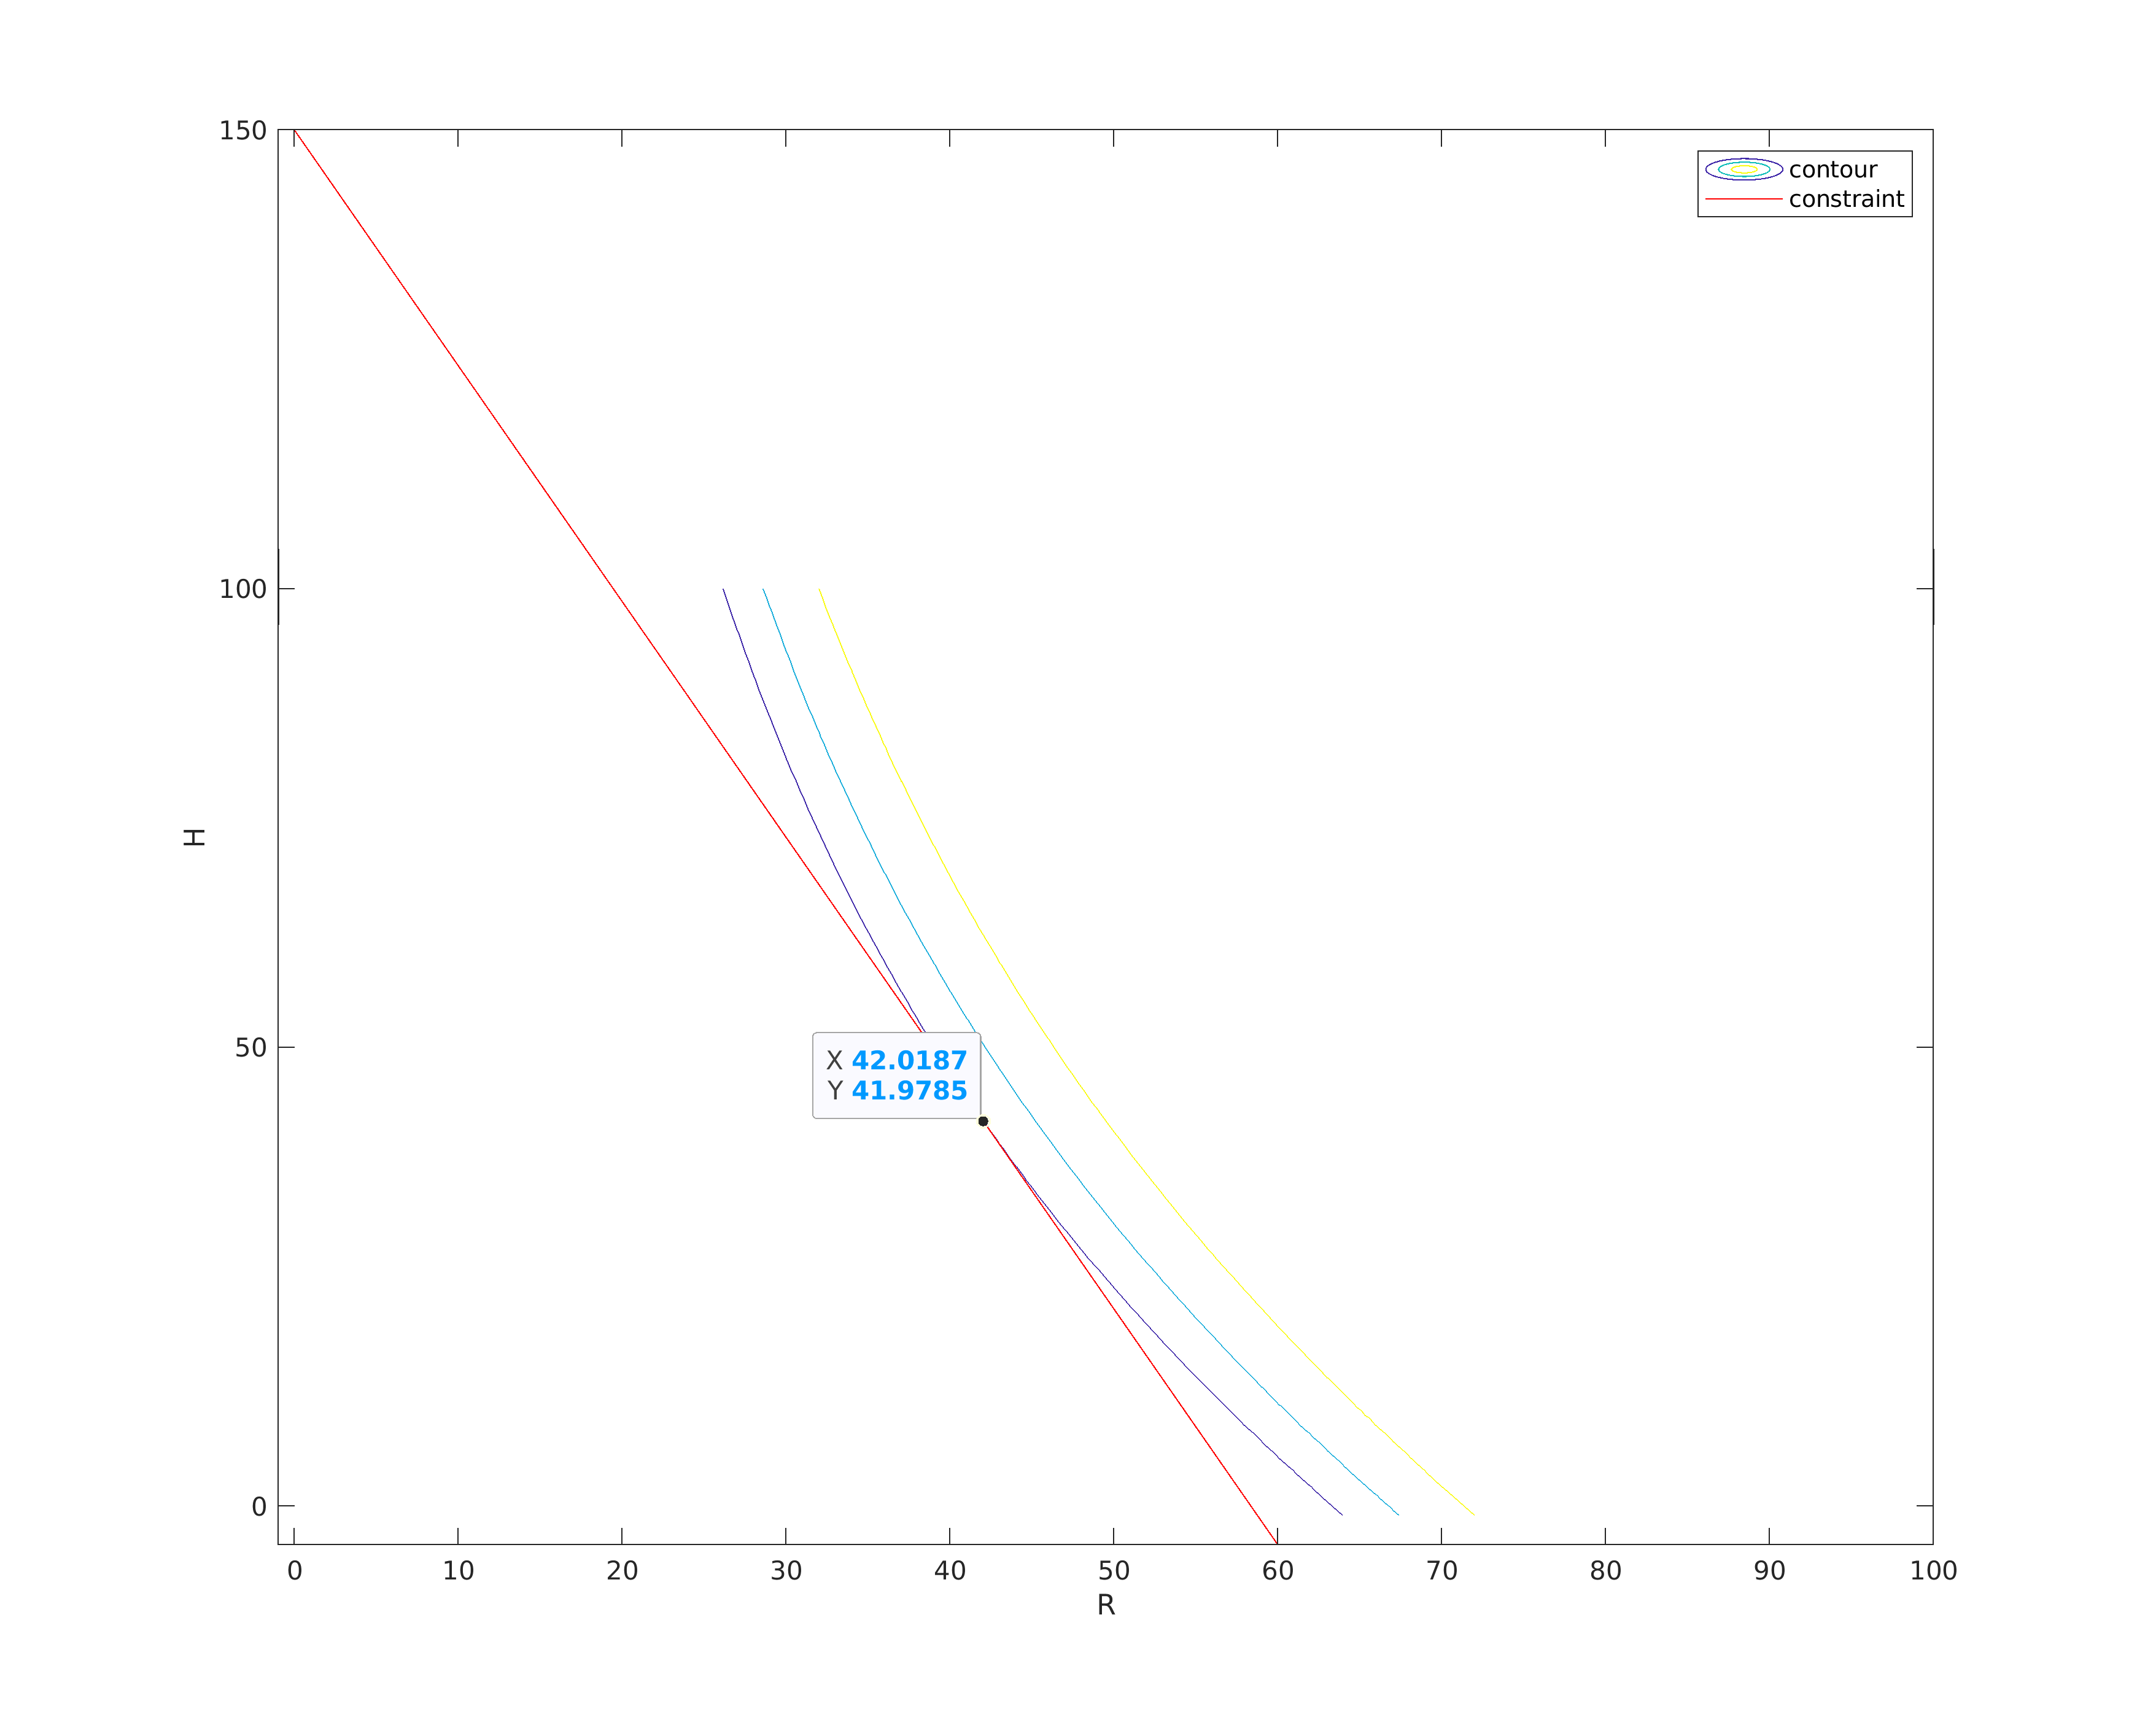
\includegraphics[width=0.9\textwidth]{img/foo.png}
  \captionsetup{justification=centering}
  \caption{Contours of the objective function and constraint equation}
\end{figure}

By inspecting the plot it can be concluded that the optimal solution to the problem is approximately as follows:
\begin{align}
R &= 42 \\
H &= 42
\end{align}



\subsubsection{Part B}
Since we have a constraint not all the values have to be computed. First we rearrange the constraint function \ref{eq:constraint} as follows:
\begin{equation}
    H(R) = 150 - (\frac{\pi}{2}+1)R
    \label{eq:c2}
\end{equation}
Since the constraint function \ref{eq:c2} reduces the dimension of the problem we only have to compute the values of the objective function on a single line. Random points are generated by using 'rand' function of MATLAB. Total of 100000 different points is generated in the region of interest $ R \in [0, 60] $. Then, the maximum computed value is found by 'max' function of the MATLAB. The optimum of these points as follows:
\begin{align}
R &= 42.0079 \\
H &= 42.0062
\end{align}

Note that since the numbers are generated randomly the result will be different for every execution of the code.

\subsubsection{Part C}

To solve the optimization problem, I have decided to use MATLAB's 'fmincon' function, I utilized its constrained optimization features. I started by defining the objective function to minimize and providing initial variable guesses. Then, I specified the constraints, including the equality condition. By following this approach, I successfully obtained a solution by leveraging the power of MATLAB's optimization capabilities. The result is as follows:

\begin{align}
R &= 42.0074 \\
H &= 42.0074
\end{align}

We can see that the graphical solution, random search method and the built in MATLAB function found the same solution.

\newpage
\subsubsection{Code}
\lstinputlisting[style=Matlab-editor, basicstyle=\mlttfamily\scriptsize]{Q3.m}

\newpage

\subsection{Question 4}
\subsubsection{Methodology}
The code follows a steepest descent method to solve Rosenbrock's "banana function" test problem. This iterative optimization approach aims to find the minimum of the function by iteratively updating the current point. The update is performed by moving in the direction of steepest descent, which is determined by the gradient of the function at each point.

The termination criteria in the code determine when to stop the iterations. One of the criteria is based on a tolerance level. The code calculates the relative error by comparing the change in function value between consecutive iterations. If this error falls below a specified tolerance level, the iterations are terminated as the solution is considered to have converged.

Additionally, the code tracks the minimum function value encountered during the iterations. If the function value at a certain iteration is lower than the minimum function value found so far, it updates the minimum value and resets a counter. However, if the counter exceeds a certain threshold, indicating a lack of improvement, the iterations are terminated.

By combining the termination criteria based on the tolerance level and the counter for lack of improvement, the code ensures that the iterations continue until either the solution converges or there is no significant improvement in the function value. This approach strikes a balance between accuracy and convergence speed, allowing the code to find a reasonably optimal solution within a given number of iterations.

Overall, the code implements a simplified steepest descent method to solve Rosenbrock's "banana function" test problem. The termination criteria based on the tolerance level and the counter for lack of improvement provide control over the convergence of the solution, ensuring a balance between accuracy and convergence speed.

\newpage

\subsubsection{Results}

\begin{figure}[H]
  \centering
  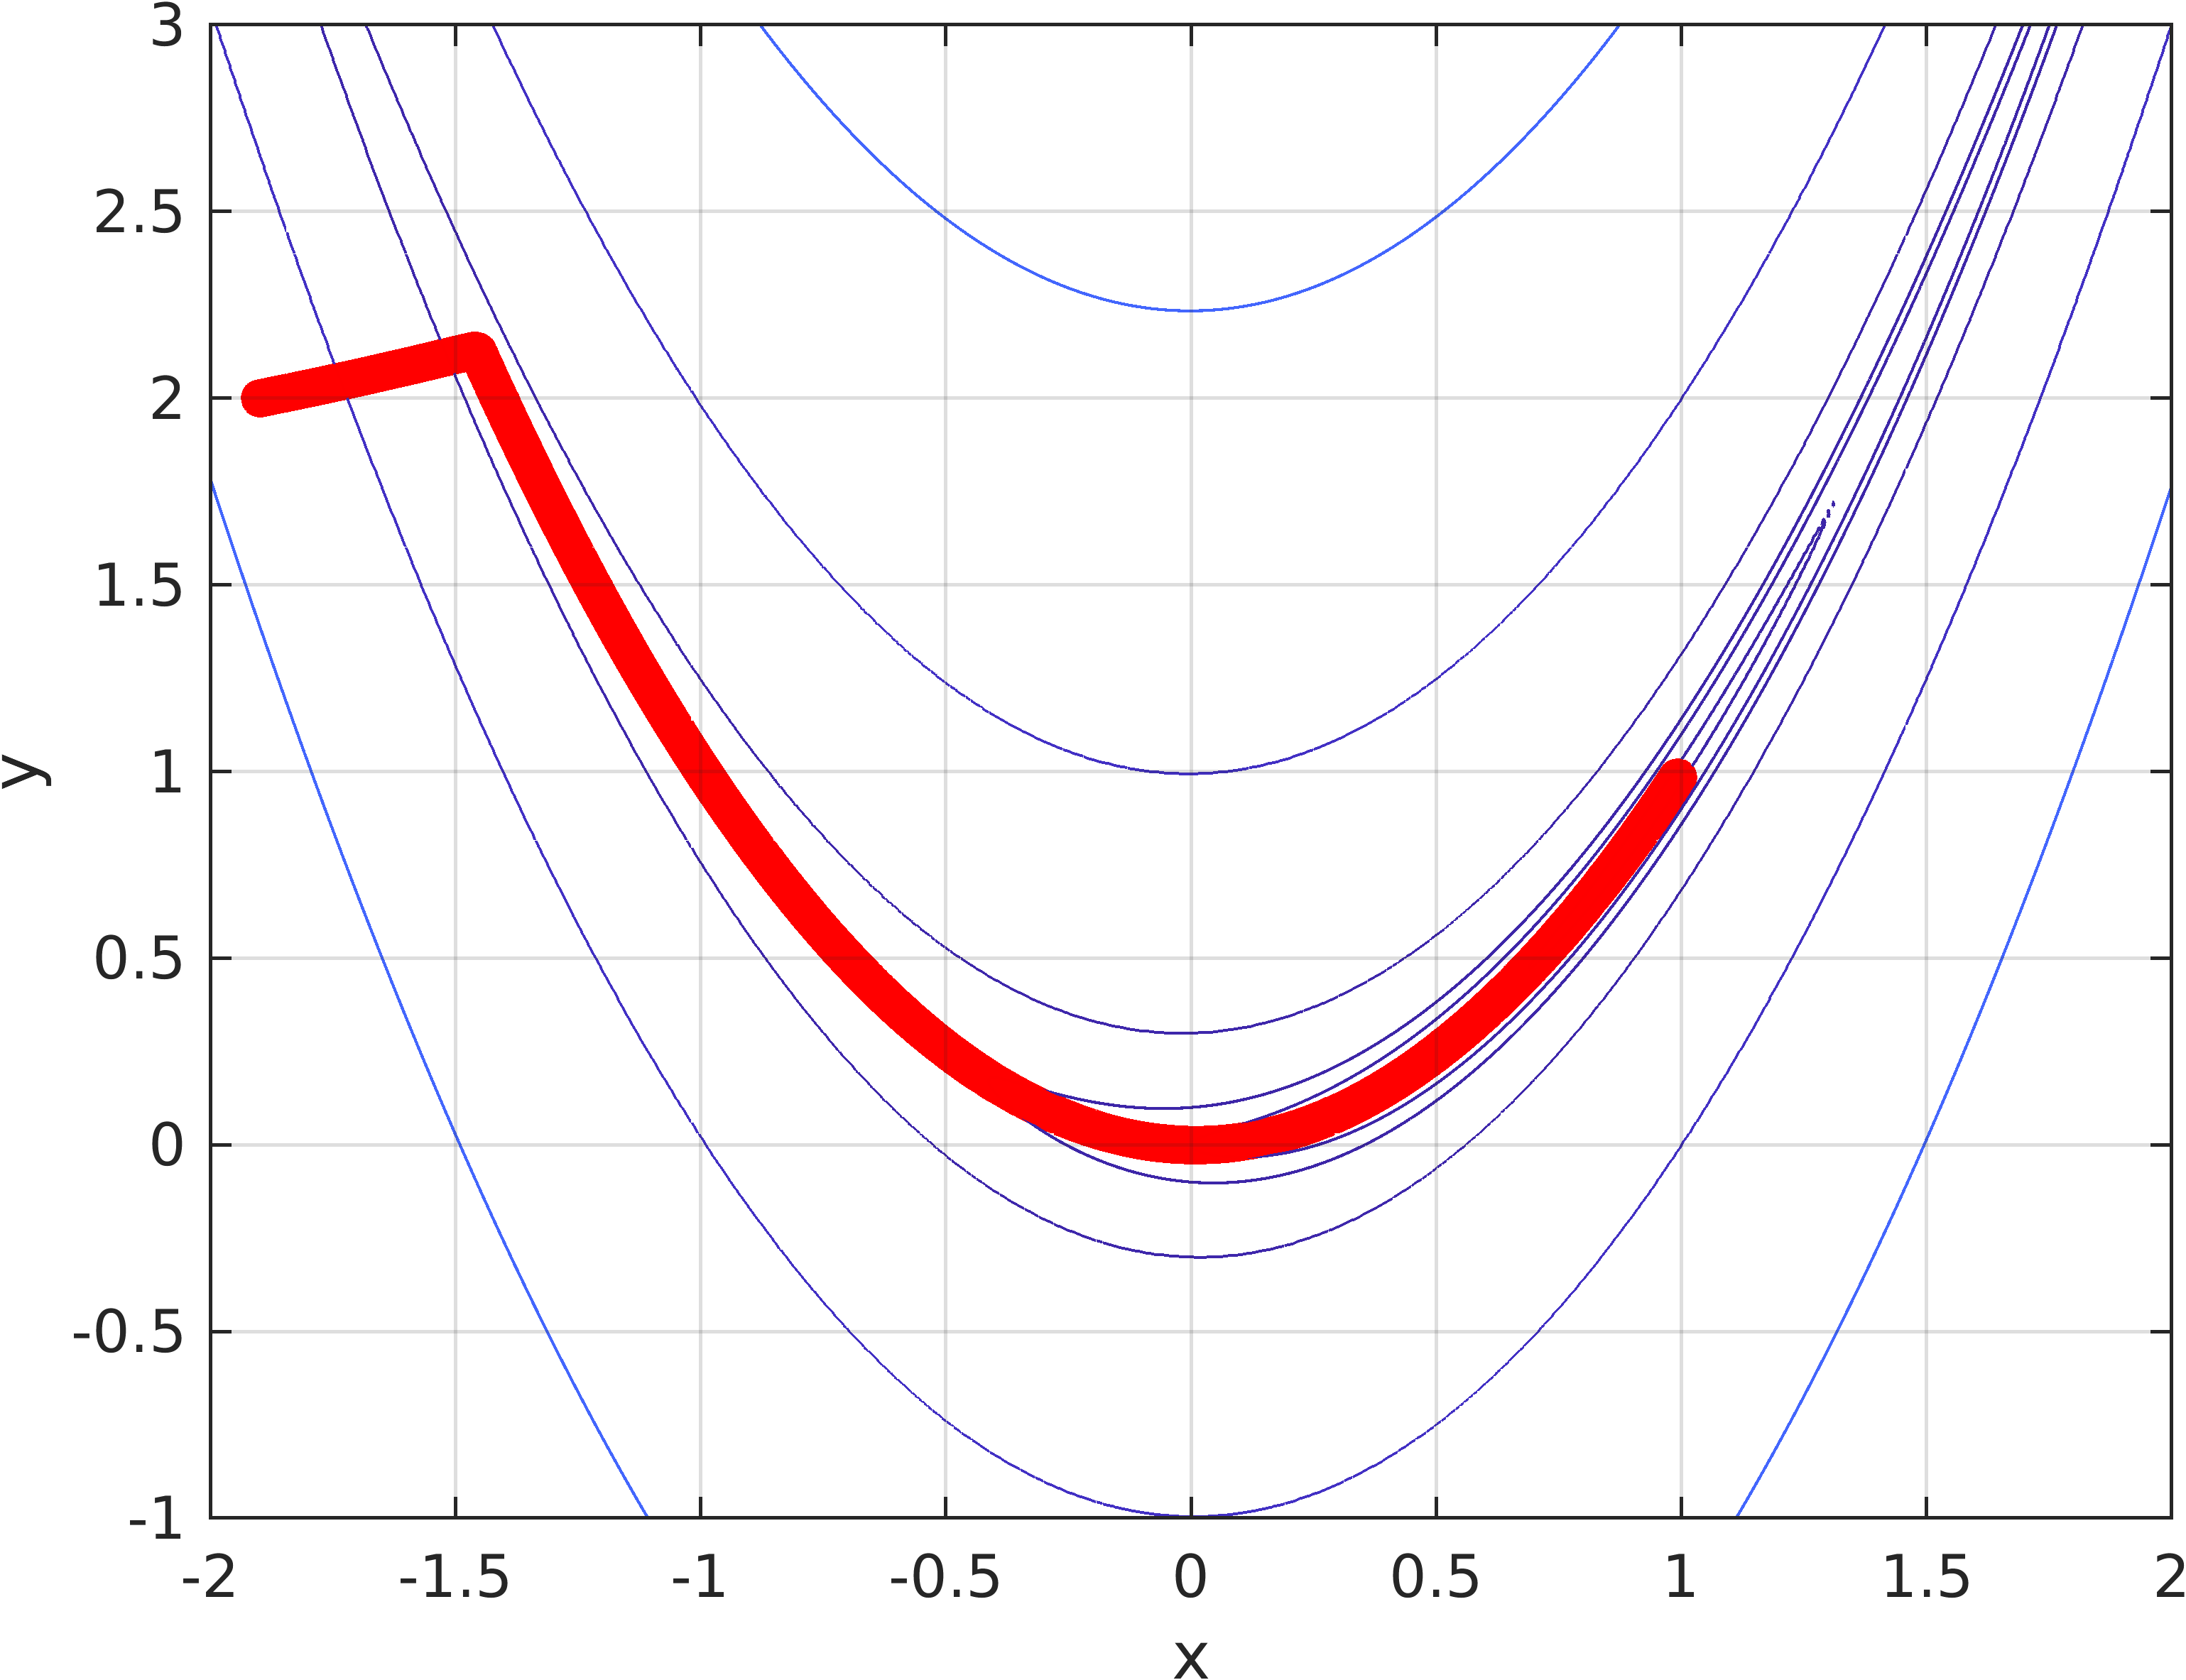
\includegraphics[width=0.8\textwidth]{img/path.png}
  \captionsetup{justification=centering}
  \caption{Contours and the path of iterations}
\end{figure}

The generated plot presents a contour representation of the Rosenbrock's "banana function" test problem. The contour lines are spaced as in handout 6. Not all the contours are shown because if so the contours cover whole figure and the figure can not be readable. Overlaid on the contour plot are dots that represent the solution at each step of the optimization process. These dots depict the progression of the algorithm and demonstrate the path followed from the initial guess to the final solution. Due to the numerous iterations, the dots appear connected, resembling lines rather than individual points.

The connected dots form a trajectory that reveals the optimization algorithm's path throughout the optimization process. The trajectory originates from the initial guess and proceeds in the direction of steepest descent, aiming to locate the minimum of the function. The length and shape of the trajectory provide insights into the convergence behavior of the algorithm and reflect the landscape of the function itself. By observing the optimization path, it becomes possible to understand how the algorithm navigates the contours of the function to find the optimal solution.
\vspace{10}

\begin{figure}[H]
  \centering
  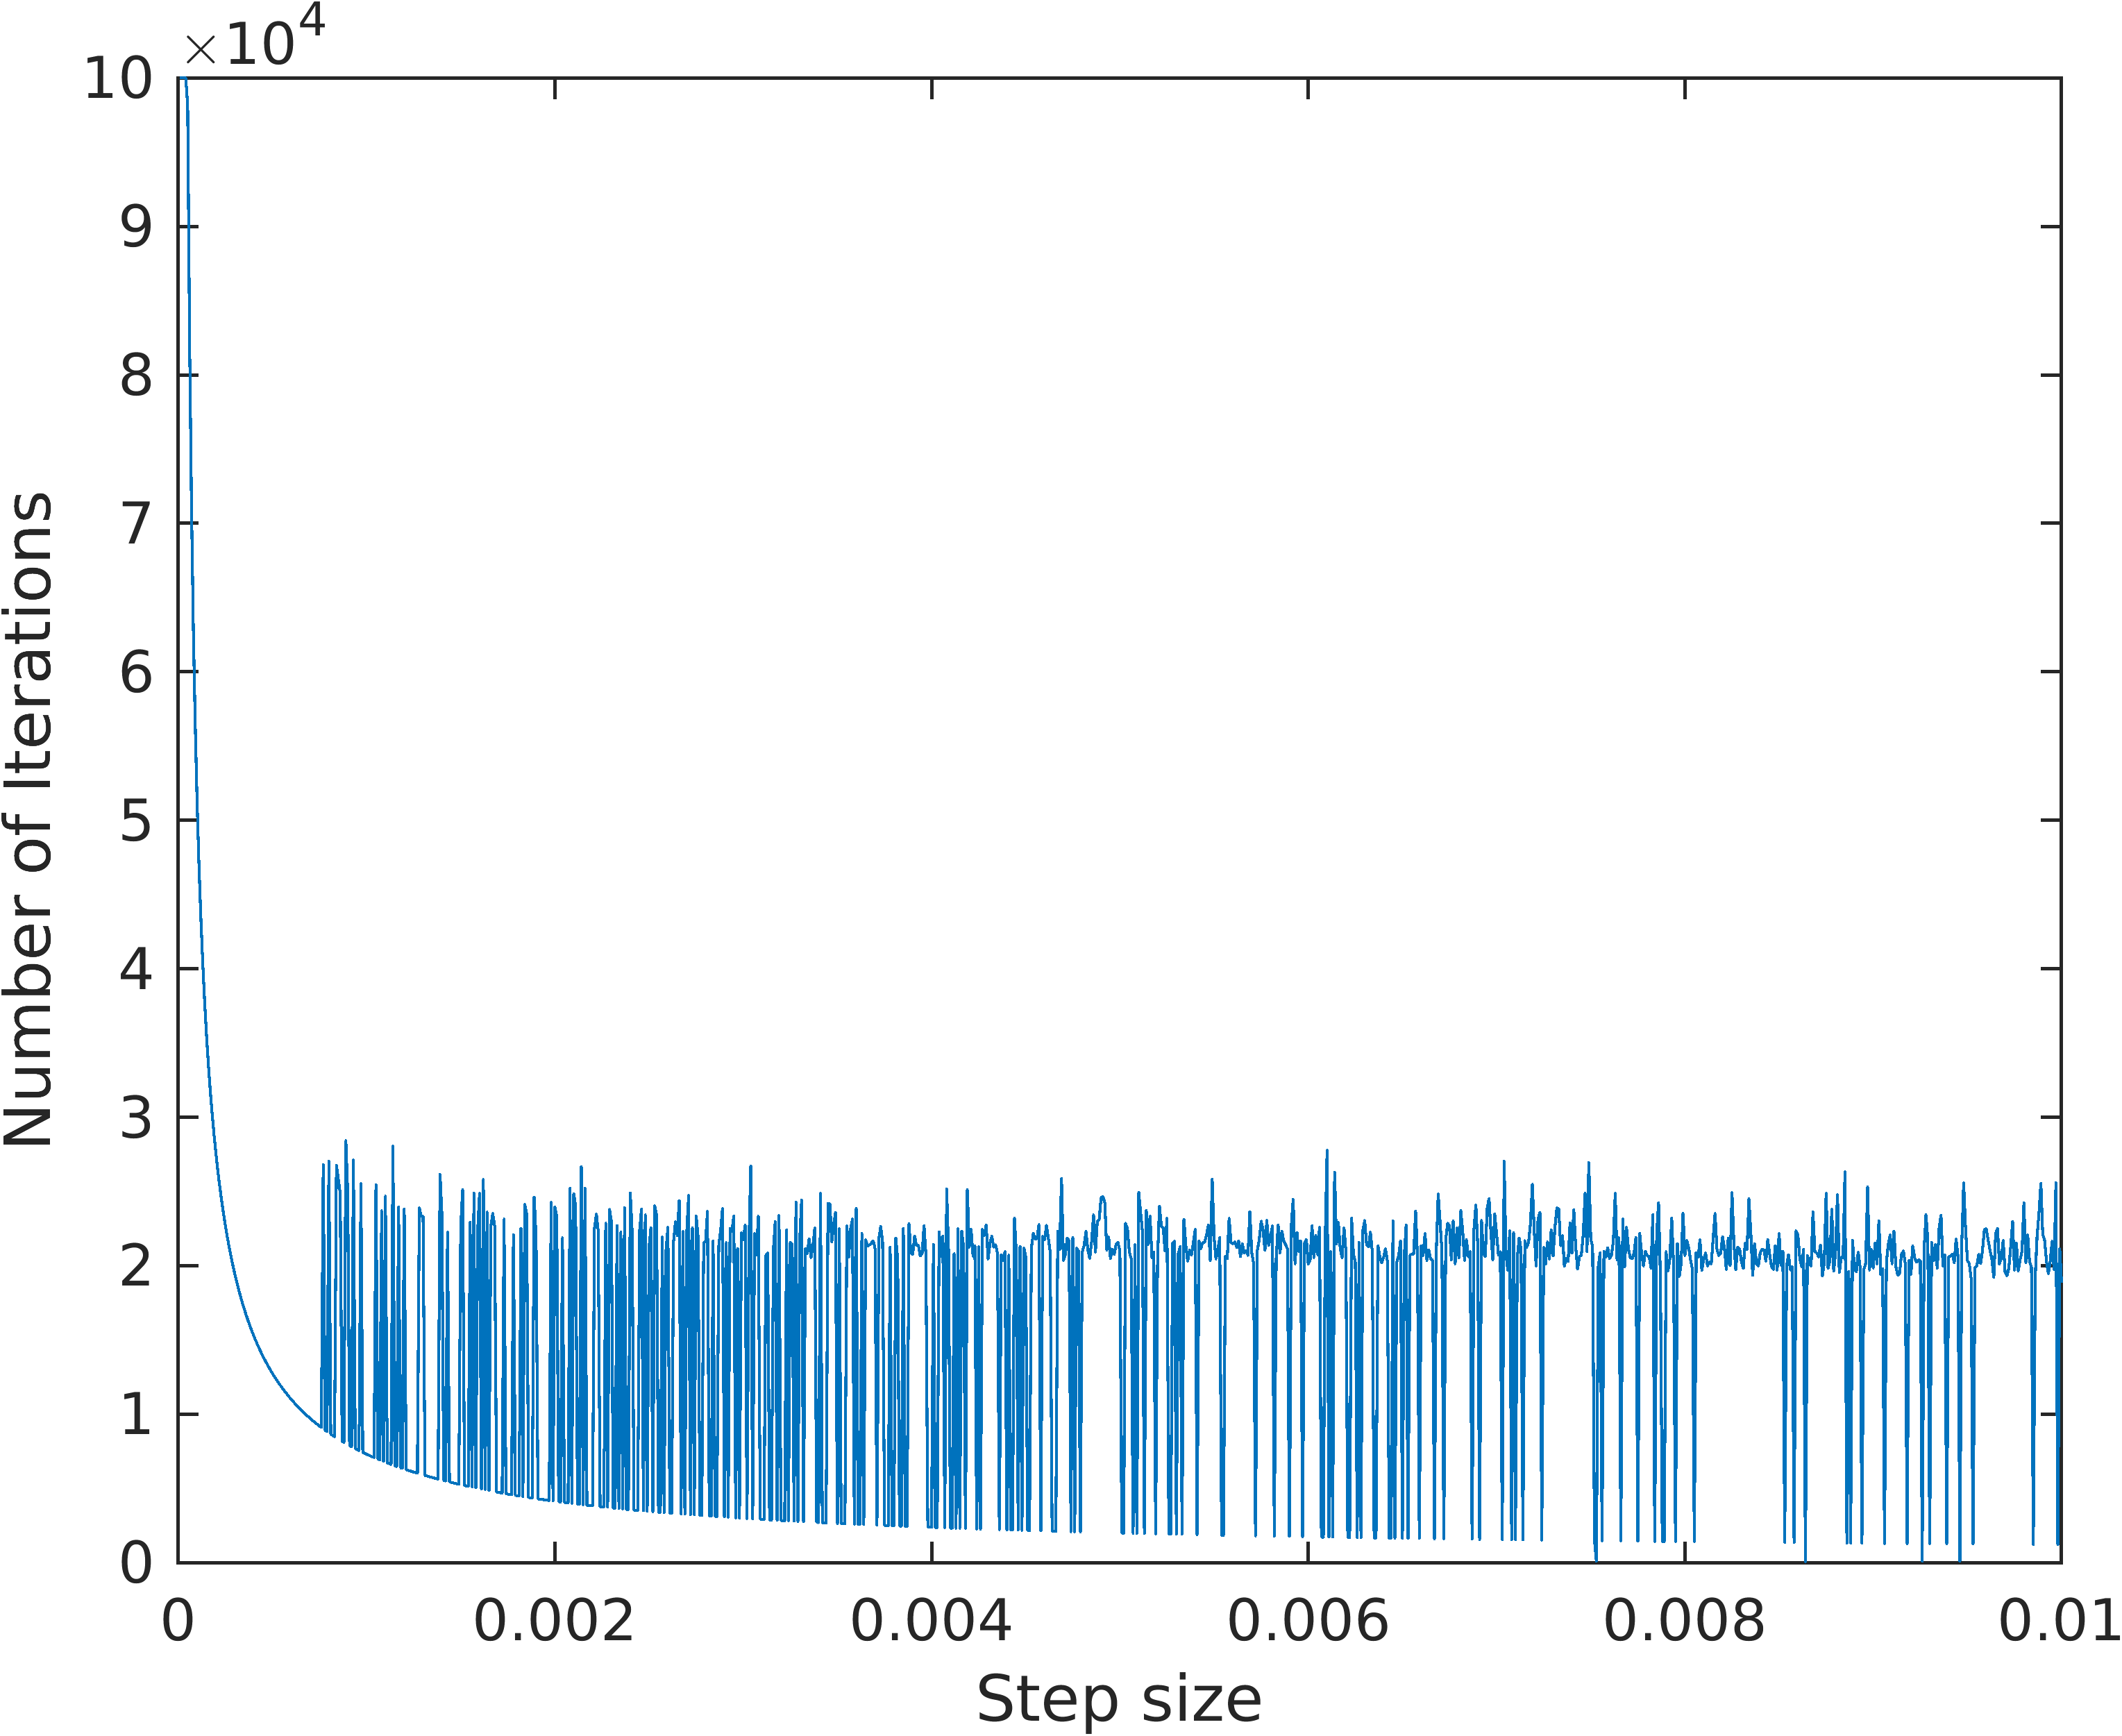
\includegraphics[width=0.8\textwidth]{img/stepvsnof.png}
  \captionsetup{justification=centering}
  \caption{Step size versus number of iterations}
\end{figure}

The variations in the number of iterations observed for specific step sizes in the provided data can be attributed to the complex nature of the function being optimized and the characteristics of the optimization method employed. The function exhibits intricate patterns and peculiar behavior, which can pose challenges for traditional optimization algorithms. In this case, the optimization approach utilized encounters difficulties in achieving convergence within a reasonable number of iterations for certain step sizes.

The irregularities in the convergence pattern are indicative of the algorithm struggling to navigate the intricate landscape of the function. Due to the steep and narrow nature of the function's valley, the algorithm's search process is hindered, resulting in inefficient convergence. The step sizes used in the optimization method play a crucial role in determining the algorithm's progress. If the step size is excessively large, the algorithm tends to overshoot the optimal point, leading to an increased number of iterations required for convergence. Conversely, excessively small step sizes impede progress and necessitate a higher number of iterations to reach the optimal point. In our case as we can see from the plot as the step size passes some thresholds the algorithm starts to overshoot the optimum point and the lack of improvement counter starts. If the algorithm does not have the necessary improvement the process is terminated. That is the main reason why we see some zigzag patterns on the plot because the overshoot might cause the number of iterations to increase significantly.

To address this challenge, it is beneficial to dynamically adjust the step size throughout the optimization process. Techniques such as line search or backtracking can be employed to identify an optimal step size at each iteration, taking into account the local properties of the function and the gradient information. This adaptive step size adjustment aids the algorithm in effectively navigating the intricate valley, thereby enhancing convergence speed.

In summary, the fluctuations in the number of iterations associated with specific step sizes reflect the difficulties encountered by the optimization method when applied to the complex function in question. Employing adaptive step size adjustment techniques can mitigate these challenges and improve the overall convergence behavior of the algorithm.

\begin{figure}[H]
  \centering
  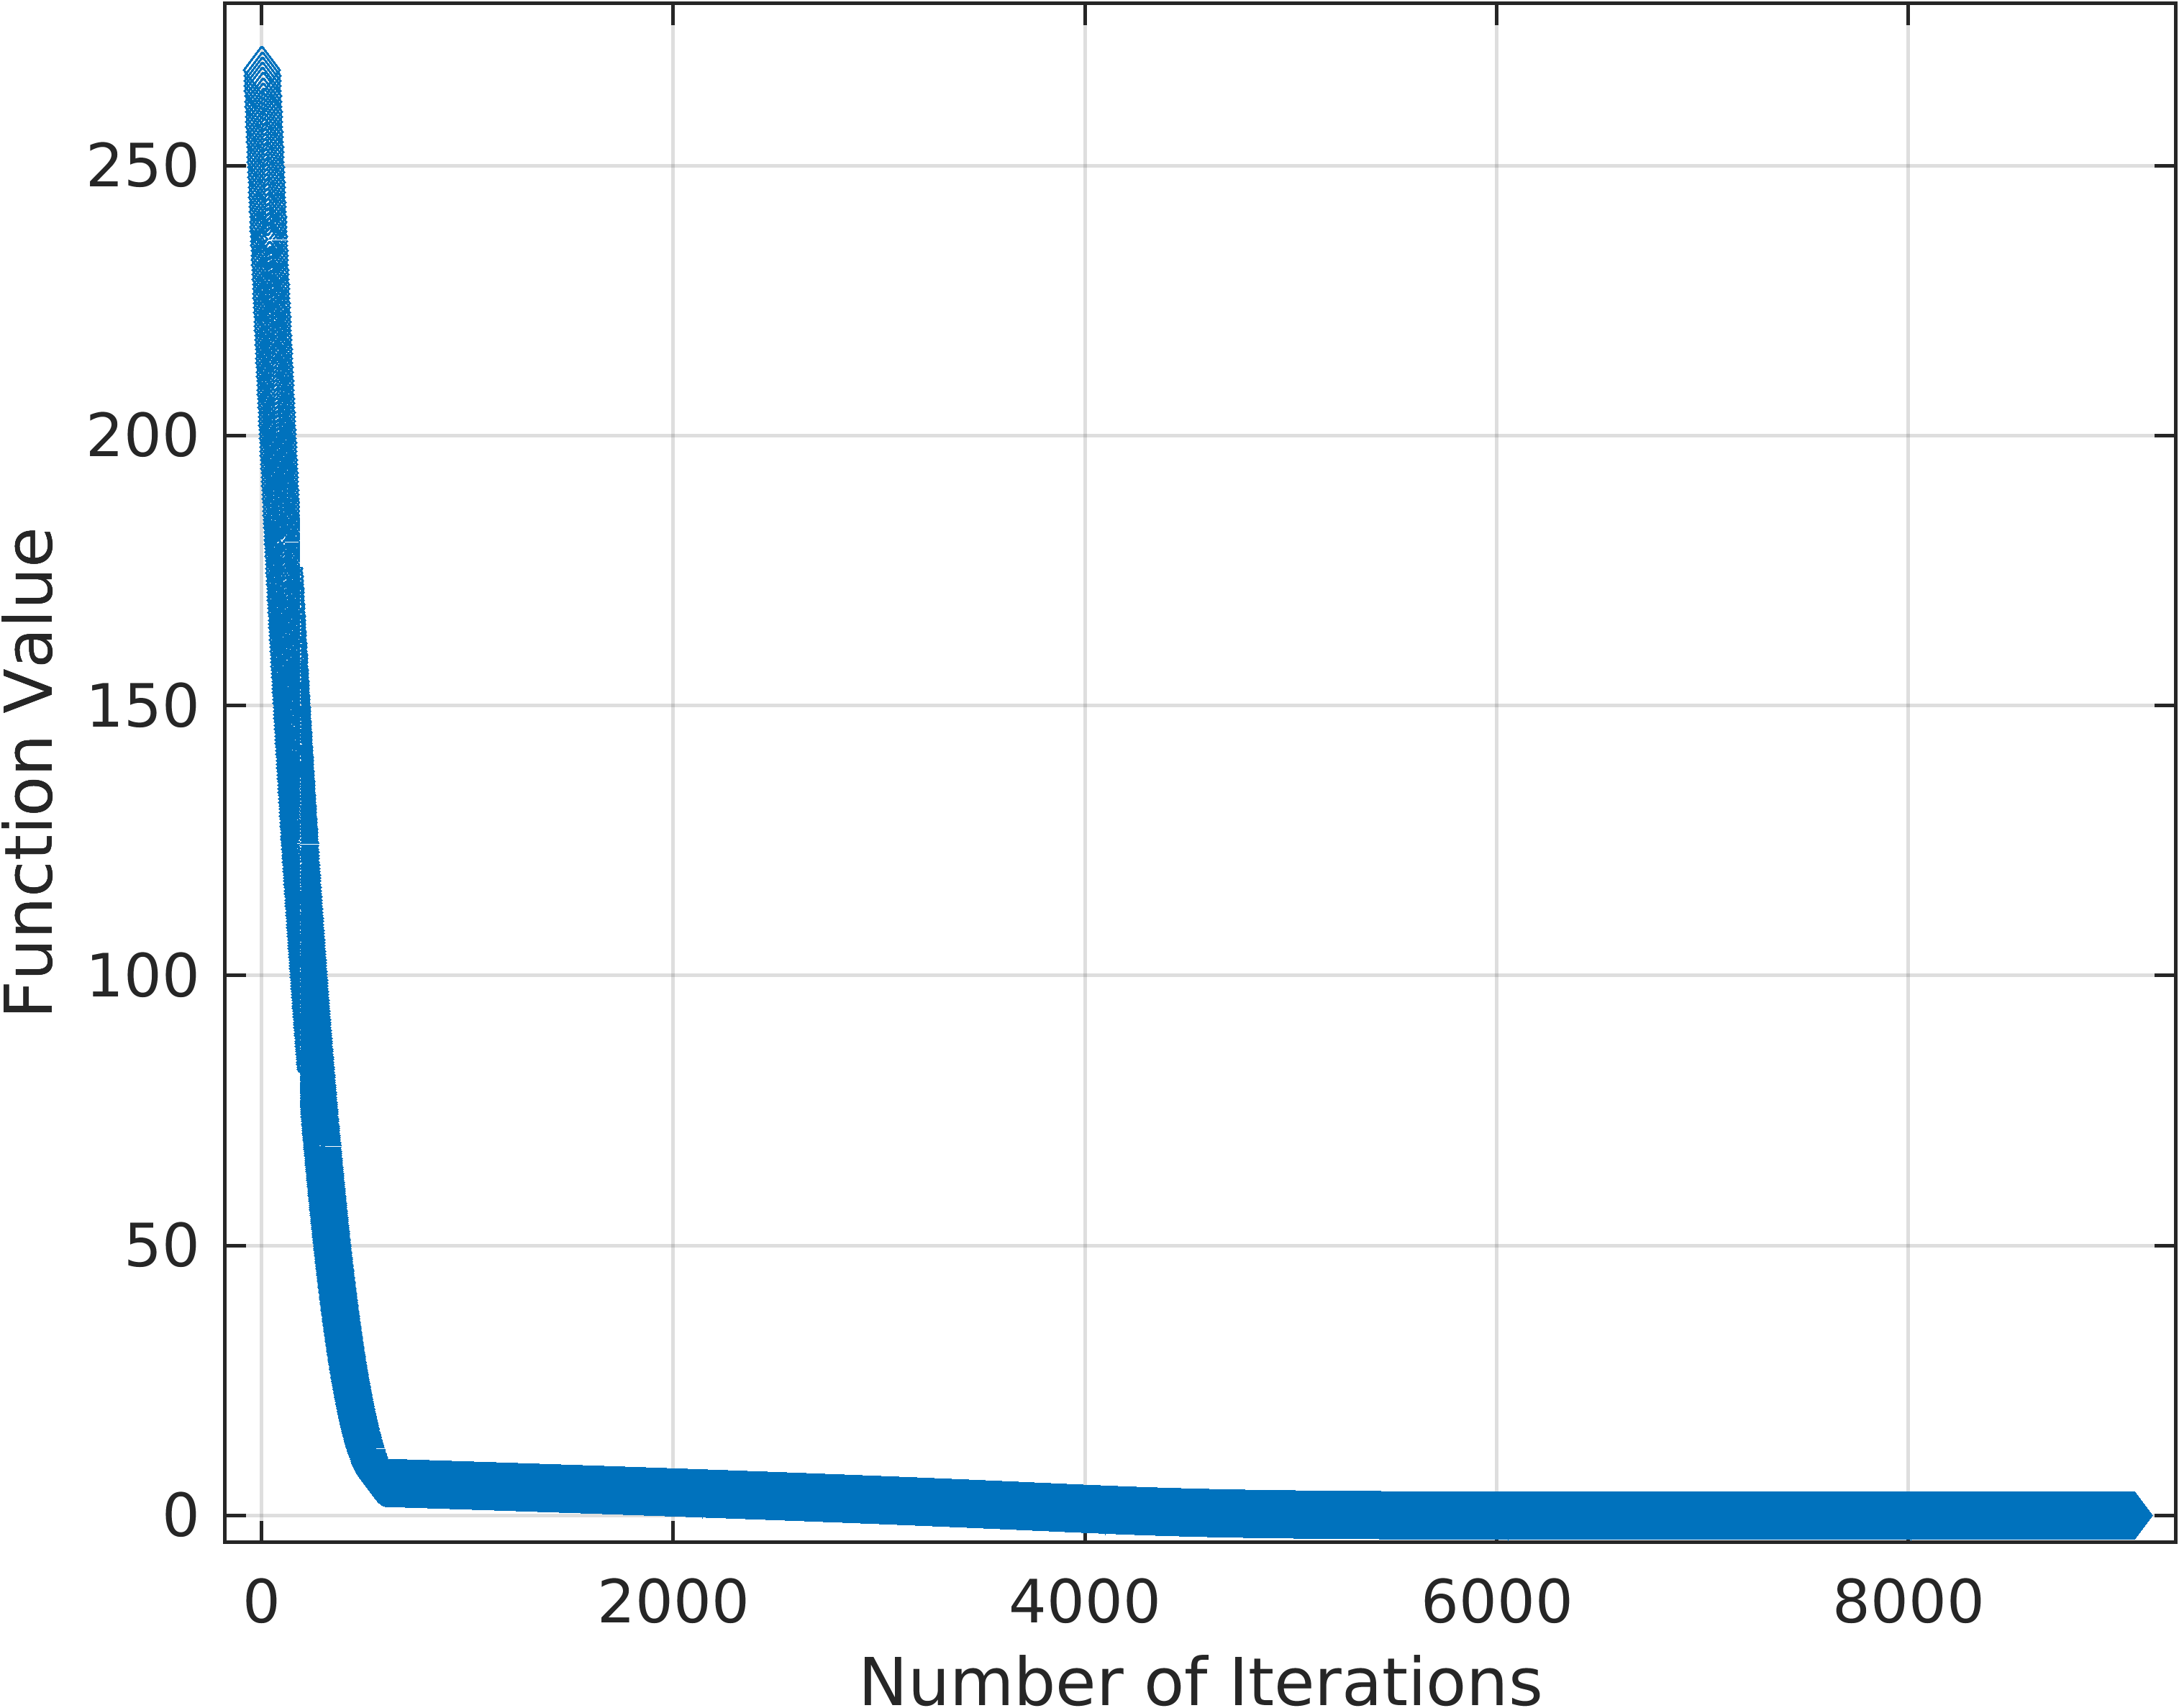
\includegraphics[width=0.8\textwidth]{img/fvsiter.png}
  \captionsetup{justification=centering}
  \caption{Number of iteration versus function value for step size 0.00076}
\end{figure}


Initially, there is a rapid descent evident in the first few hundred iterations, suggesting substantial progress in reaching the optimal solution. However, what follows is a rather sluggish convergence, which can be attributed to the inherently challenging nature of this particular test problem.

The "banana function" test problem is notorious for its intricate characteristics, including a narrow and curved valley, which poses significant hurdles for optimization algorithms. Despite the promising early progress depicted in the figure, the subsequent slow convergence clearly highlights the algorithm's struggles to navigate and achieve satisfactory results within this complex landscape.

The sharp drop observed in the initial iterations signifies the algorithm's capability to make significant advancements at the outset. However, the subsequent slow convergence pattern indicates that the algorithm encounters obstacles and faces difficulties in fine-tuning the solution to its optimal state.


\newpage
\subsubsection{Code}
\lstinputlisting[style=Matlab-editor, basicstyle=\mlttfamily\scriptsize]{Q4.m}

\newpage
\section{Discussion}

For the second question. The analysis conducted using a 'golden section search,' presented a systematic approach to narrowing down the interval in which the maximum growth rate of the function occurs. Through a series of repeated iterations, this method successfully reduced the interval size until achieving a desirable level of precision. The effectiveness of this method became apparent as it reliably found the optimal value. Another approach, referred to as the 'quadratic interpolation method,' involved the approximation of the function using a quadratic polynomial. This method iteratively updated the interval based on the obtained values. Lastly, the 'Newton's method' demonstrated a notable characteristic of rapid convergence towards the optimal solution when given a proper initial guess which was not the case on our case. The given initial guess resulted in a divergence for both exact and approximated derivatives. When we give a closer initial guess the method was the fastest method. In summary, each method possesses distinct advantages and considerations. The selection of a specific method depends on the particular requirements and constraints of the problem at hand. By understanding the unique attributes of each approach, researchers and practitioners can make informed choices to tackle optimization challenges effectively. For the third question the acquisition was the creation of the objective functions and evaluating them by using constraints. This achieved by using graphical solution, random serach and the built in MATLAB functions. For the fourth question the aim was to construact a gradient based optimization code. By observing the solution paths generated by the code, it becomes evident that the choice of step size is a trade-off between accuracy and speed. Smaller step sizes provide more precise solutions but require a larger number of iterations, while larger step sizes expedite the convergence but risk missing finer details of the function. Therefore, it is essential to select an appropriate step size based on the specific problem at hand, balancing the desired level of accuracy with computational efficiency.

\section{Conclusion}


In conclusion, the analysis presented in this discussion revealed several methods for optimization. The 'golden section search' proved to be a systematic approach for narrowing down intervals, while the 'quadratic interpolation method' involved approximating functions with polynomials. 'Newton's method' demonstrated convergence towards the optimal solution but required a suitable initial guess. The acquisition of objective functions and evaluation involved graphical solutions, random search, and MATLAB functions. Constructing a gradient-based optimization code required careful consideration of step size, balancing accuracy and speed. Overall, understanding the unique characteristics of each method and selecting appropriate techniques is crucial for effective optimization. Researchers and practitioners can make informed choices to tackle challenges based on specific requirements and constraints.


\end{document}
